%
% ruecken2.tex -- Ruecken für das Buch
%
% (c) 2018-2025 Prof Dr Andreas Müller, Hochschule Rapperswil
%
\documentclass[11pt]{standalone}
\usepackage{tikz}
\usepackage{times}
\usepackage{geometry}
\usepackage[utf8]{inputenc}
\usepackage[T1]{fontenc}
\usepackage{times}
\usepackage{amsmath,amscd}
\usepackage{amssymb}
\usepackage{amsfonts}
\usepackage{german}
\usepackage{txfonts}
\usepackage{ifthen}
\usepackage{qrcode}
\usetikzlibrary{math}
\geometry{papersize={417mm,278mm},total={417mm,278mm},top=72.27pt, bottom=0pt, left=72.27pt, right=0pt}
\newboolean{guidelines}
\setboolean{guidelines}{true}
\setboolean{guidelines}{false}
\newboolean{teilnehmer}
\setboolean{teilnehmer}{false}
\setboolean{teilnehmer}{true}

\begin{document}
\begin{tikzpicture}[>=latex, scale=1]

\tikzmath{
        real \ruecken, \einschlag, \gelenk, \breite, \hoehe;
        \ruecken = 3.5;
        \einschlag = 1.6;
        \gelenk = 0.8;
        \breite = 16.7;
        \hoehe = 24.6;
        real \bogengreite, \bogenhoehe;
        \bogenbreite = 2 * (\breite + \einschlag + \gelenk) + \ruecken;
        \bogenhoehe = 2 * \einschlag + \hoehe;
}

\clip ({0.46*\bogenbreite},-1) rectangle
	({0.54*\bogenbreite},{0.48*\bogenhoehe+1});

\node at ({0.75*\bogenbreite},8.0)
	{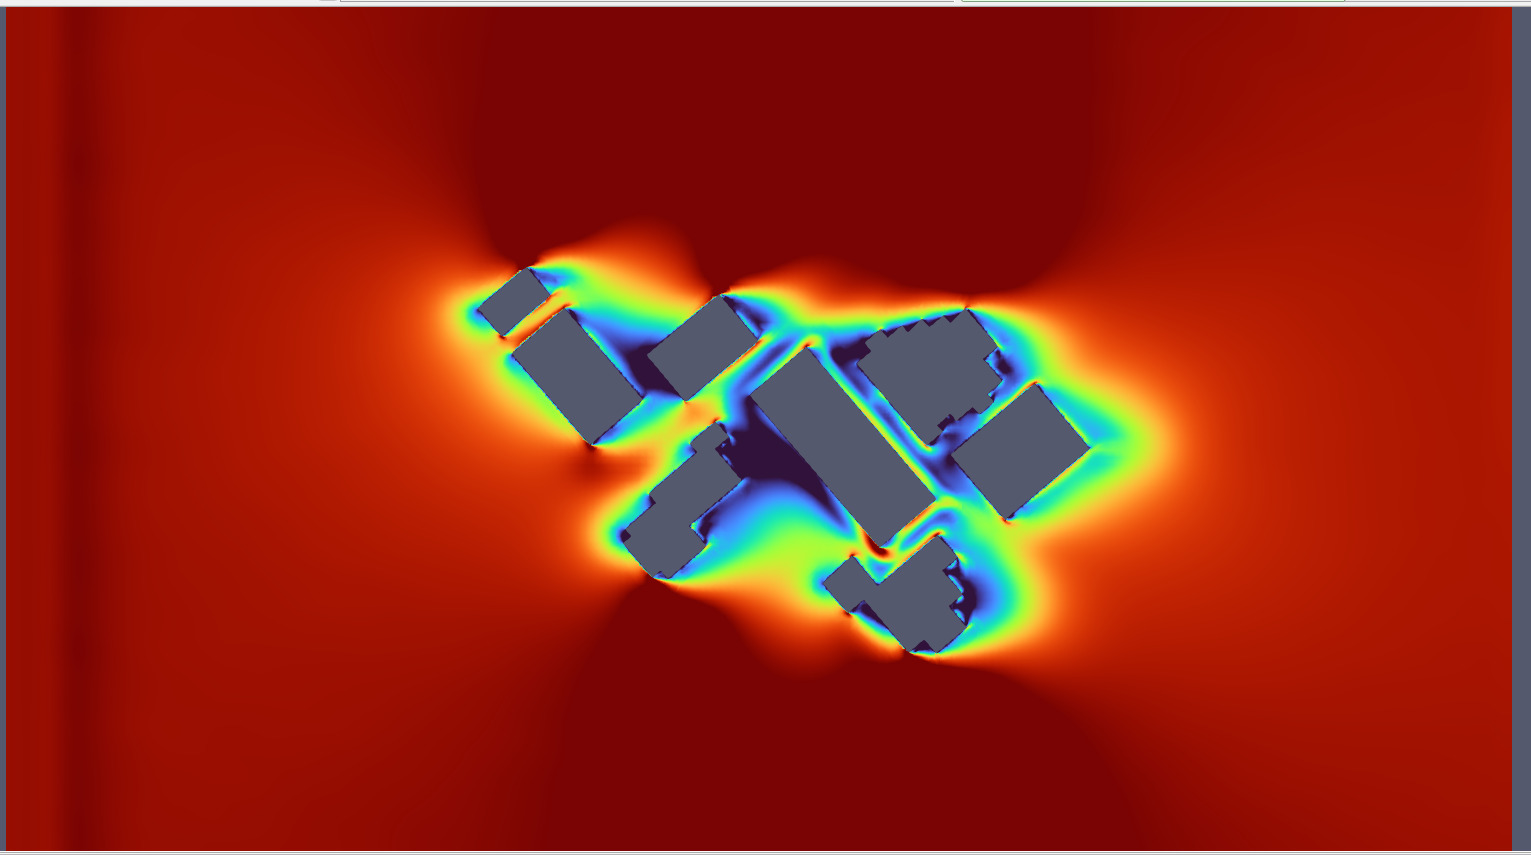
\includegraphics[width=38cm]{frontimage.jpg}};

\end{tikzpicture}
\end{document}
